\documentclass[11pt]{article}
\usepackage[textwidth=18.0cm, textheight=23.0cm, top=2.0cm]{geometry}
\usepackage{pst-all}
\usepackage{amssymb}
\usepackage{tikz}
\usepackage{underscore}\begin{document}
\pagestyle{empty}


ClassName: \underline{\textbf{Class_05.2bp-26}}
\par
BinSize: \underline{\textbf{100 × 100}}
\par
ReduceSize: \underline{\textbf{100 × 100}}
\par
TypeNum: \underline{\textbf{60}}
\par
Num: \underline{\textbf{60}}
\par
OutS: \underline{\textbf{140000}}
\par
InS: \underline{\textbf{124587}}
\par
Rate: \underline{\textbf{0.890}}
\par
UB: \underline{\textbf{14}}
\par
LB0: \underline{\textbf{14}}
\par
LB: \underline{\textbf{14}}
\par
LBWithCut: \underline{\textbf{14}}
\par
NodeCut: \underline{\textbf{0}}
\par
ExtendedNodeCnt: \underline{\textbf{1}}
\par
GenNodeCnt: \underline{\textbf{1}}
\par
PrimalNode: \underline{\textbf{0}}
\par
ColumnCount: \underline{\textbf{14}}
\par
TotalCutCount: \underline{\textbf{0}}
\par
RootCutCount: \underline{\textbf{0}}
\par
LPSolverCnt: \underline{\textbf{1}}
\par
PricingSolverCnt: \underline{\textbf{0}}
\par
BranchAndBoundNum: \underline{\textbf{1}}
\par
isOpt: \underline{\textbf{true}}
\par
TimeOnInitSolution: \underline{\textbf{600.000 s}}
\par
TimeOnPrimal: \underline{\textbf{0.000 s}}
\par
TimeOnPricing: \underline{\textbf{0.000 s}}
\par
TimeOnRmp: \underline{\textbf{0.062 s}}
\par
TotalTime: \underline{\textbf{600.375 s}}
\par
\newpage


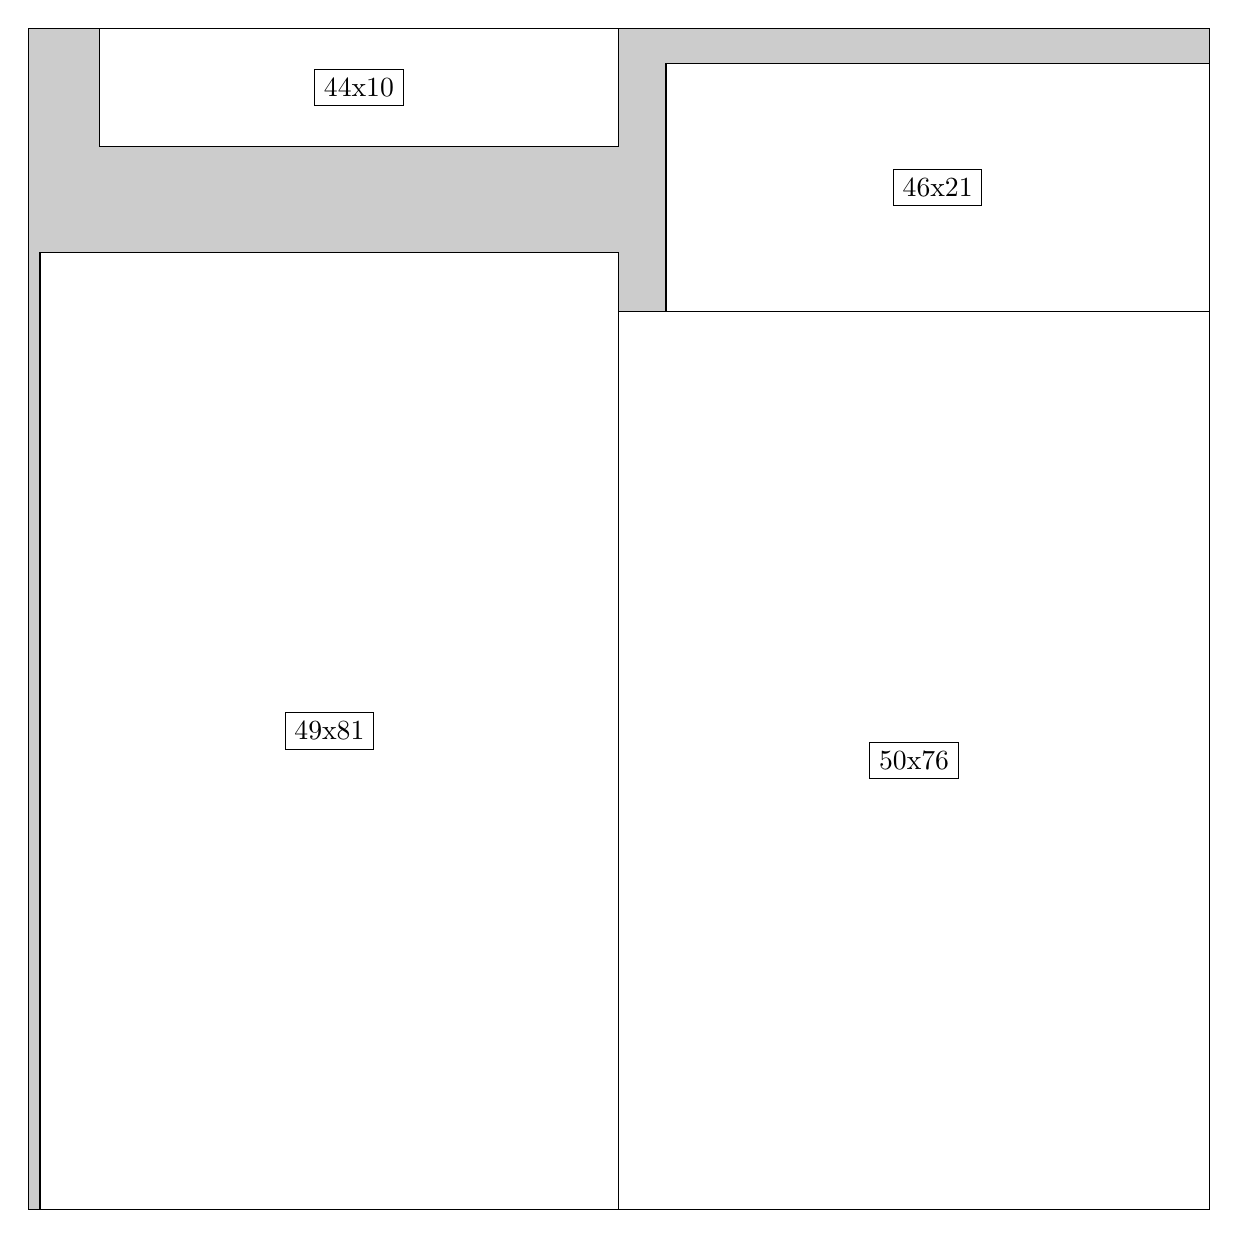
\begin{tikzpicture}[shorten >=1pt,scale=1.0,every node/.style={scale=1.0},->]
\tikzstyle{vertex}=[circle,fill=black!25,minimum size=14pt,inner sep=0pt]
\filldraw[fill=gray!40!white, draw=black] (0,0) rectangle (15.0,15.0);
\foreach \name/\x/\y/\w/\h in {50x76/7.5/0.0/7.5/11.4,46x21/8.1/11.4/6.8999999999999995/3.15,49x81/0.15/0.0/7.35/12.15,44x10/0.8999999999999999/13.5/6.6/1.5}
\filldraw[fill=white!40!white, draw=black] (\x,\y) rectangle node[draw] (\name) {\name} ++(\w,\h);
\end{tikzpicture}


w =50 , h =76 , x =50 , y =0 , v =3800
\par
w =46 , h =21 , x =54 , y =76 , v =966
\par
w =49 , h =81 , x =1 , y =0 , v =3969
\par
w =44 , h =10 , x =6 , y =90 , v =440
\par
\newpage


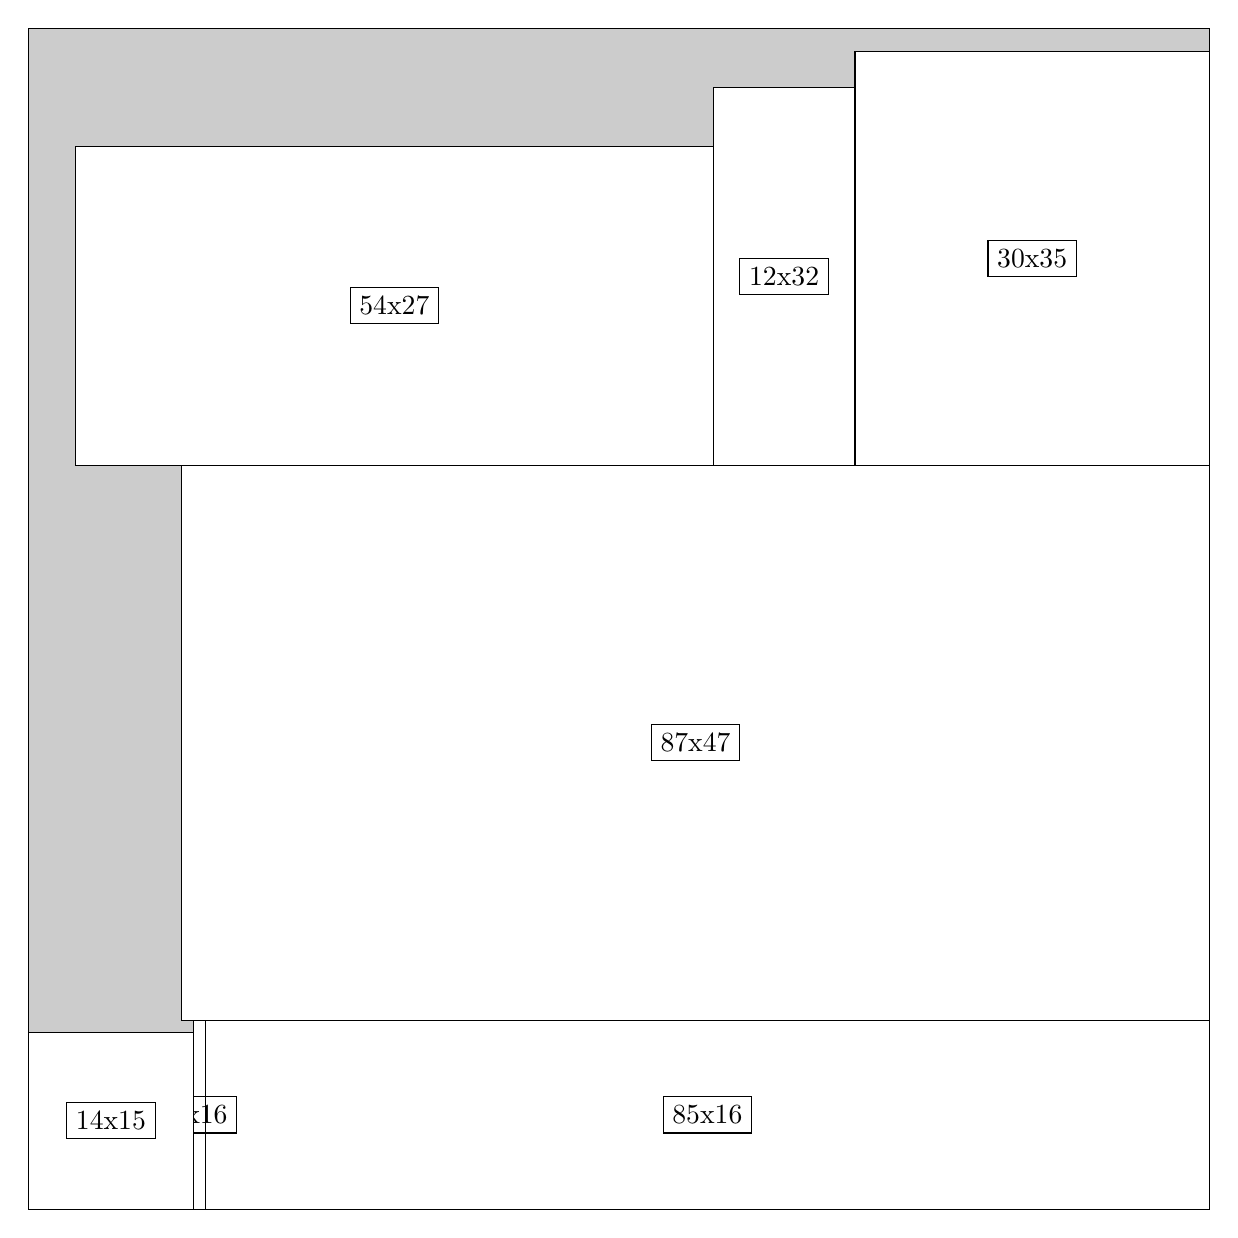
\begin{tikzpicture}[shorten >=1pt,scale=1.0,every node/.style={scale=1.0},->]
\tikzstyle{vertex}=[circle,fill=black!25,minimum size=14pt,inner sep=0pt]
\filldraw[fill=gray!40!white, draw=black] (0,0) rectangle (15.0,15.0);
\foreach \name/\x/\y/\w/\h in {85x16/2.25/0.0/12.75/2.4,1x16/2.1/0.0/0.15/2.4,14x15/0.0/0.0/2.1/2.25,87x47/1.95/2.4/13.049999999999999/7.05,30x35/10.5/9.45/4.5/5.25,12x32/8.7/9.45/1.7999999999999998/4.8,54x27/0.6/9.45/8.1/4.05}
\filldraw[fill=white!40!white, draw=black] (\x,\y) rectangle node[draw] (\name) {\name} ++(\w,\h);
\end{tikzpicture}


w =85 , h =16 , x =15 , y =0 , v =1360
\par
w =1 , h =16 , x =14 , y =0 , v =16
\par
w =14 , h =15 , x =0 , y =0 , v =210
\par
w =87 , h =47 , x =13 , y =16 , v =4089
\par
w =30 , h =35 , x =70 , y =63 , v =1050
\par
w =12 , h =32 , x =58 , y =63 , v =384
\par
w =54 , h =27 , x =4 , y =63 , v =1458
\par
\newpage


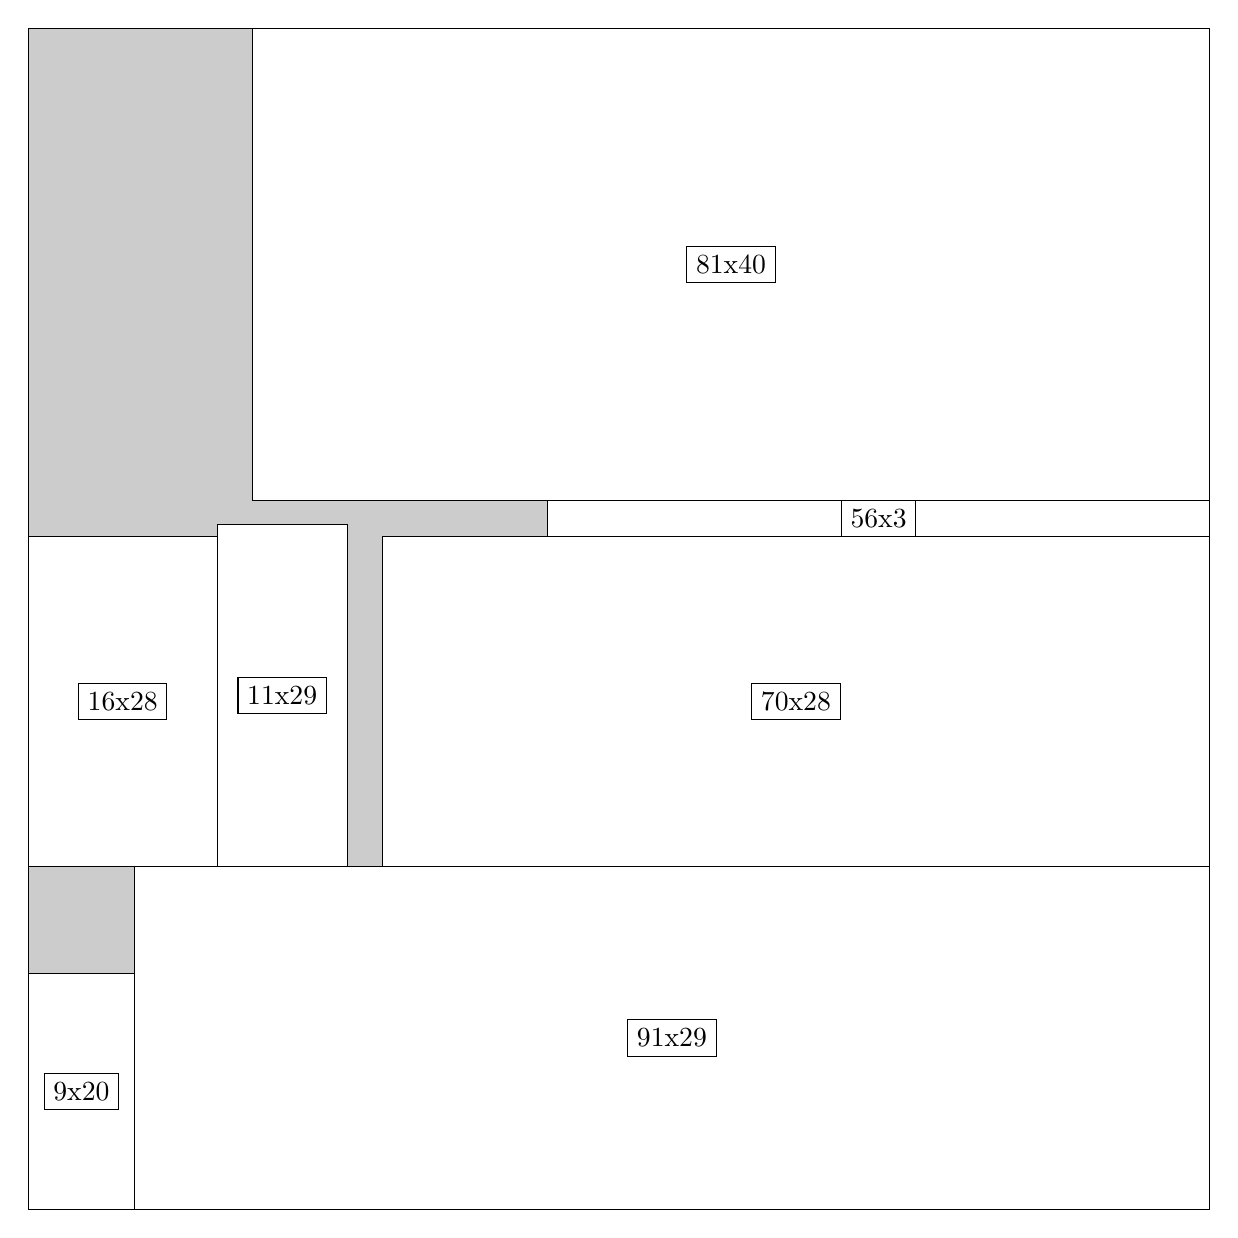
\begin{tikzpicture}[shorten >=1pt,scale=1.0,every node/.style={scale=1.0},->]
\tikzstyle{vertex}=[circle,fill=black!25,minimum size=14pt,inner sep=0pt]
\filldraw[fill=gray!40!white, draw=black] (0,0) rectangle (15.0,15.0);
\foreach \name/\x/\y/\w/\h in {91x29/1.3499999999999999/0.0/13.65/4.35,9x20/0.0/0.0/1.3499999999999999/3.0,70x28/4.5/4.35/10.5/4.2,56x3/6.6/8.549999999999999/8.4/0.44999999999999996,11x29/2.4/4.35/1.65/4.35,16x28/0.0/4.35/2.4/4.2,81x40/2.85/9.0/12.15/6.0}
\filldraw[fill=white!40!white, draw=black] (\x,\y) rectangle node[draw] (\name) {\name} ++(\w,\h);
\end{tikzpicture}


w =91 , h =29 , x =9 , y =0 , v =2639
\par
w =9 , h =20 , x =0 , y =0 , v =180
\par
w =70 , h =28 , x =30 , y =29 , v =1960
\par
w =56 , h =3 , x =44 , y =57 , v =168
\par
w =11 , h =29 , x =16 , y =29 , v =319
\par
w =16 , h =28 , x =0 , y =29 , v =448
\par
w =81 , h =40 , x =19 , y =60 , v =3240
\par
\newpage


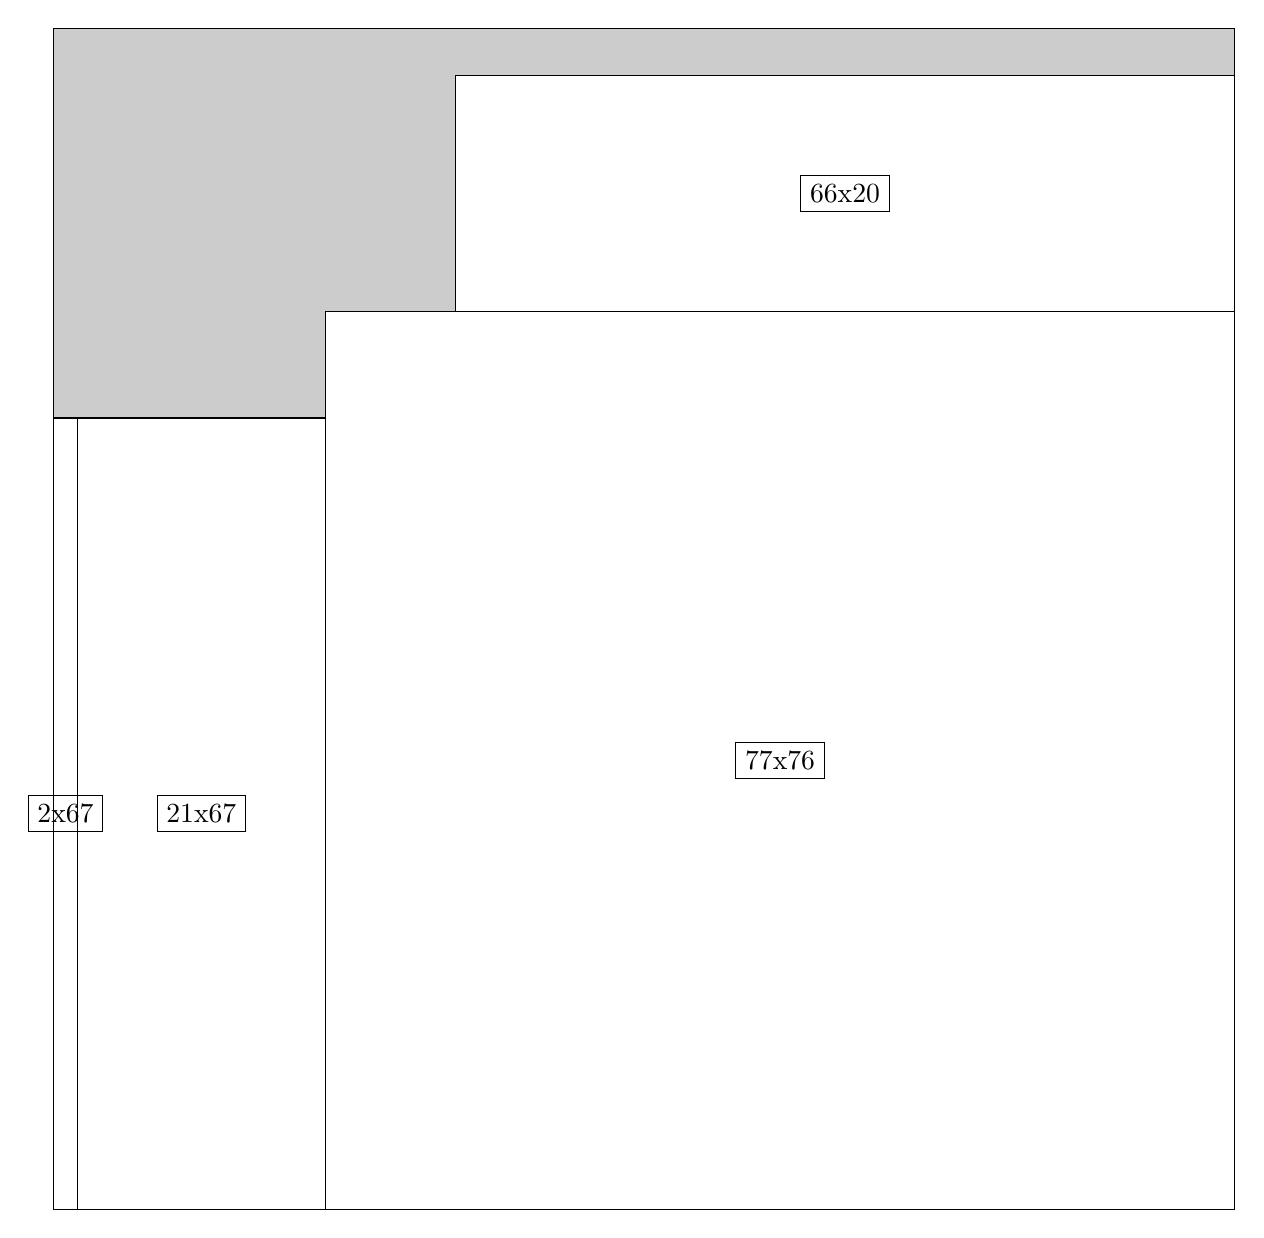
\begin{tikzpicture}[shorten >=1pt,scale=1.0,every node/.style={scale=1.0},->]
\tikzstyle{vertex}=[circle,fill=black!25,minimum size=14pt,inner sep=0pt]
\filldraw[fill=gray!40!white, draw=black] (0,0) rectangle (15.0,15.0);
\foreach \name/\x/\y/\w/\h in {77x76/3.4499999999999997/0.0/11.549999999999999/11.4,21x67/0.3/0.0/3.15/10.049999999999999,2x67/0.0/0.0/0.3/10.049999999999999,66x20/5.1/11.4/9.9/3.0}
\filldraw[fill=white!40!white, draw=black] (\x,\y) rectangle node[draw] (\name) {\name} ++(\w,\h);
\end{tikzpicture}


w =77 , h =76 , x =23 , y =0 , v =5852
\par
w =21 , h =67 , x =2 , y =0 , v =1407
\par
w =2 , h =67 , x =0 , y =0 , v =134
\par
w =66 , h =20 , x =34 , y =76 , v =1320
\par
\newpage


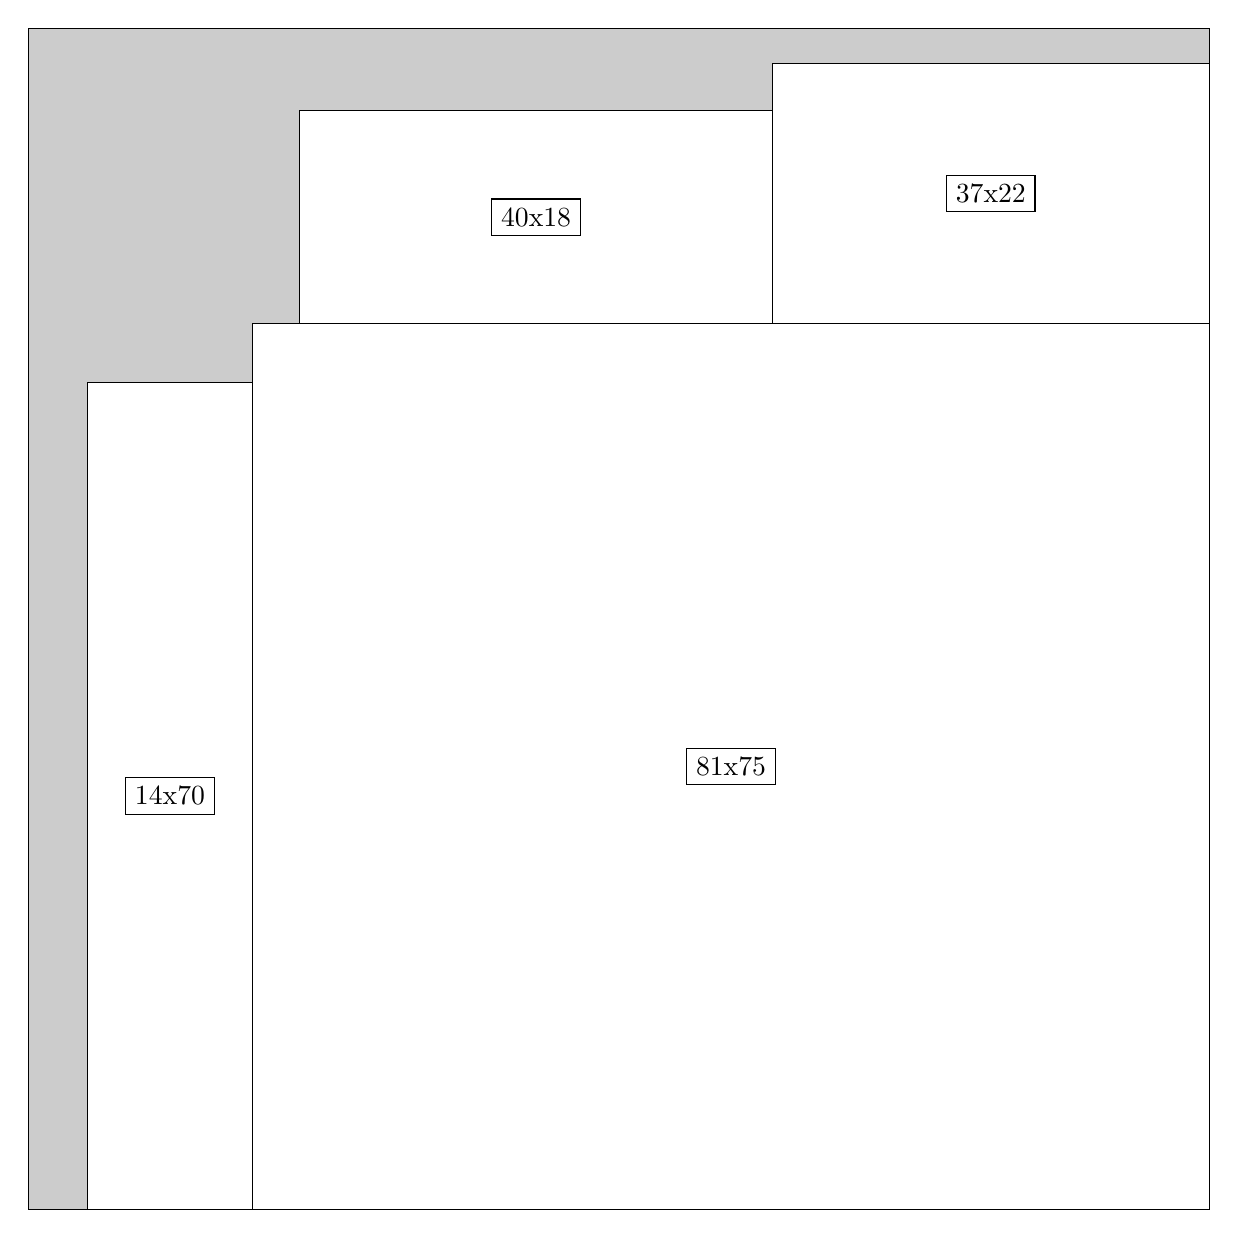
\begin{tikzpicture}[shorten >=1pt,scale=1.0,every node/.style={scale=1.0},->]
\tikzstyle{vertex}=[circle,fill=black!25,minimum size=14pt,inner sep=0pt]
\filldraw[fill=gray!40!white, draw=black] (0,0) rectangle (15.0,15.0);
\foreach \name/\x/\y/\w/\h in {81x75/2.85/0.0/12.15/11.25,14x70/0.75/0.0/2.1/10.5,37x22/9.45/11.25/5.55/3.3,40x18/3.4499999999999997/11.25/6.0/2.6999999999999997}
\filldraw[fill=white!40!white, draw=black] (\x,\y) rectangle node[draw] (\name) {\name} ++(\w,\h);
\end{tikzpicture}


w =81 , h =75 , x =19 , y =0 , v =6075
\par
w =14 , h =70 , x =5 , y =0 , v =980
\par
w =37 , h =22 , x =63 , y =75 , v =814
\par
w =40 , h =18 , x =23 , y =75 , v =720
\par
\newpage


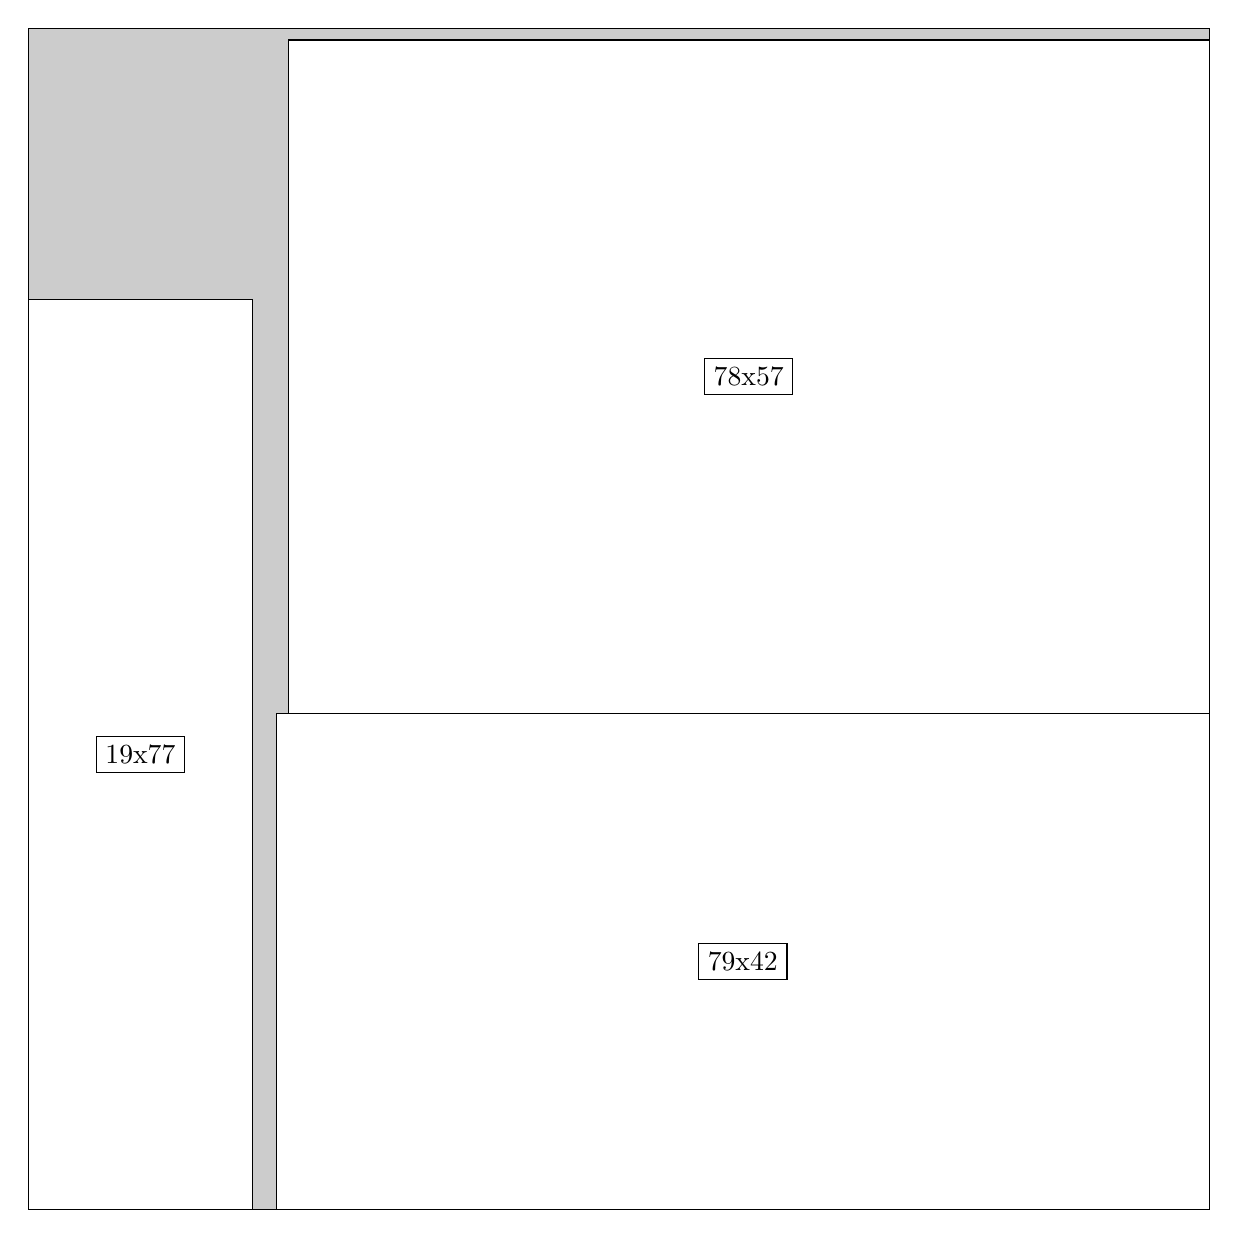
\begin{tikzpicture}[shorten >=1pt,scale=1.0,every node/.style={scale=1.0},->]
\tikzstyle{vertex}=[circle,fill=black!25,minimum size=14pt,inner sep=0pt]
\filldraw[fill=gray!40!white, draw=black] (0,0) rectangle (15.0,15.0);
\foreach \name/\x/\y/\w/\h in {79x42/3.15/0.0/11.85/6.3,78x57/3.3/6.3/11.7/8.549999999999999,19x77/0.0/0.0/2.85/11.549999999999999}
\filldraw[fill=white!40!white, draw=black] (\x,\y) rectangle node[draw] (\name) {\name} ++(\w,\h);
\end{tikzpicture}


w =79 , h =42 , x =21 , y =0 , v =3318
\par
w =78 , h =57 , x =22 , y =42 , v =4446
\par
w =19 , h =77 , x =0 , y =0 , v =1463
\par
\newpage


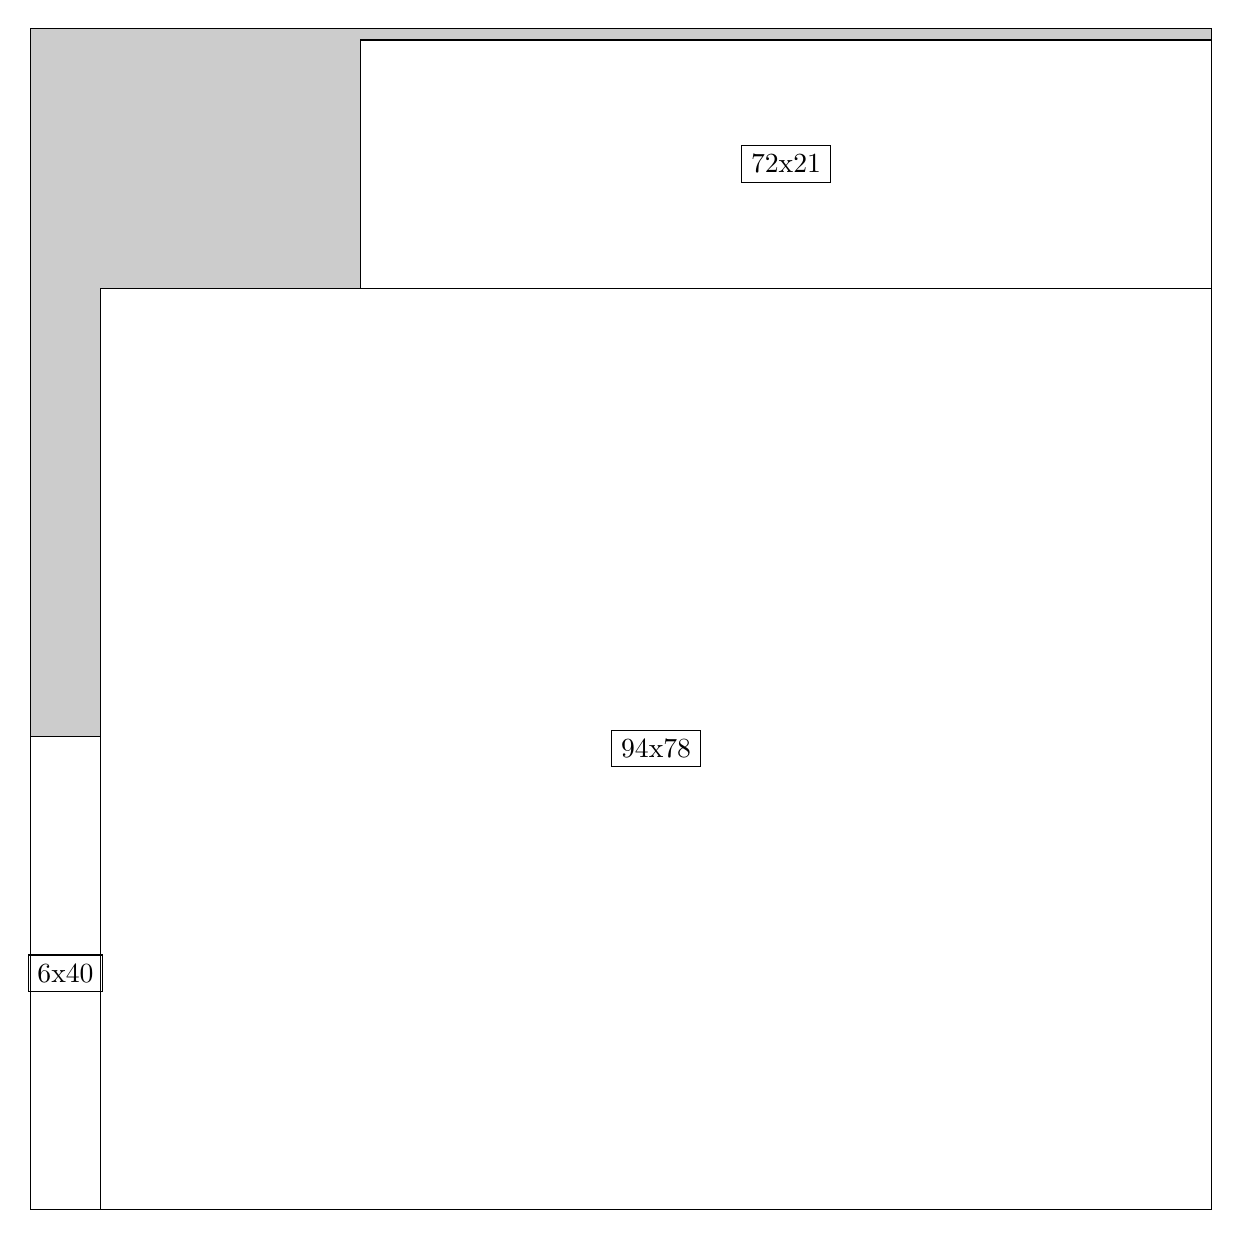
\begin{tikzpicture}[shorten >=1pt,scale=1.0,every node/.style={scale=1.0},->]
\tikzstyle{vertex}=[circle,fill=black!25,minimum size=14pt,inner sep=0pt]
\filldraw[fill=gray!40!white, draw=black] (0,0) rectangle (15.0,15.0);
\foreach \name/\x/\y/\w/\h in {94x78/0.8999999999999999/0.0/14.1/11.7,6x40/0.0/0.0/0.8999999999999999/6.0,72x21/4.2/11.7/10.799999999999999/3.15}
\filldraw[fill=white!40!white, draw=black] (\x,\y) rectangle node[draw] (\name) {\name} ++(\w,\h);
\end{tikzpicture}


w =94 , h =78 , x =6 , y =0 , v =7332
\par
w =6 , h =40 , x =0 , y =0 , v =240
\par
w =72 , h =21 , x =28 , y =78 , v =1512
\par
\newpage


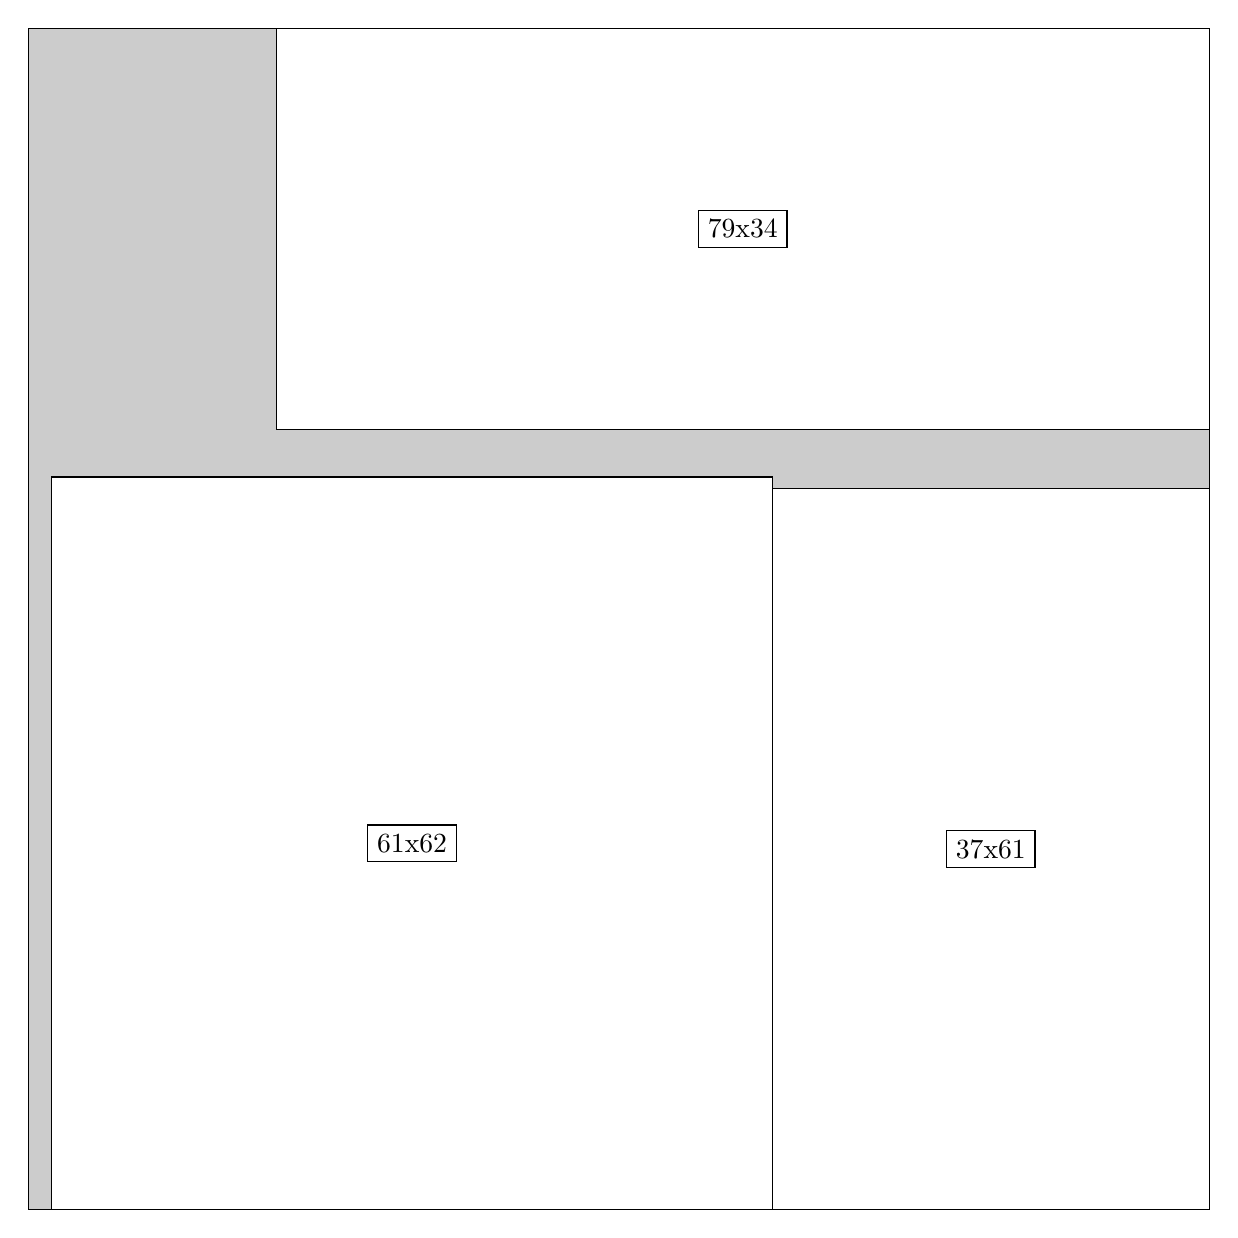
\begin{tikzpicture}[shorten >=1pt,scale=1.0,every node/.style={scale=1.0},->]
\tikzstyle{vertex}=[circle,fill=black!25,minimum size=14pt,inner sep=0pt]
\filldraw[fill=gray!40!white, draw=black] (0,0) rectangle (15.0,15.0);
\foreach \name/\x/\y/\w/\h in {37x61/9.45/0.0/5.55/9.15,61x62/0.3/0.0/9.15/9.299999999999999,79x34/3.15/9.9/11.85/5.1}
\filldraw[fill=white!40!white, draw=black] (\x,\y) rectangle node[draw] (\name) {\name} ++(\w,\h);
\end{tikzpicture}


w =37 , h =61 , x =63 , y =0 , v =2257
\par
w =61 , h =62 , x =2 , y =0 , v =3782
\par
w =79 , h =34 , x =21 , y =66 , v =2686
\par
\newpage


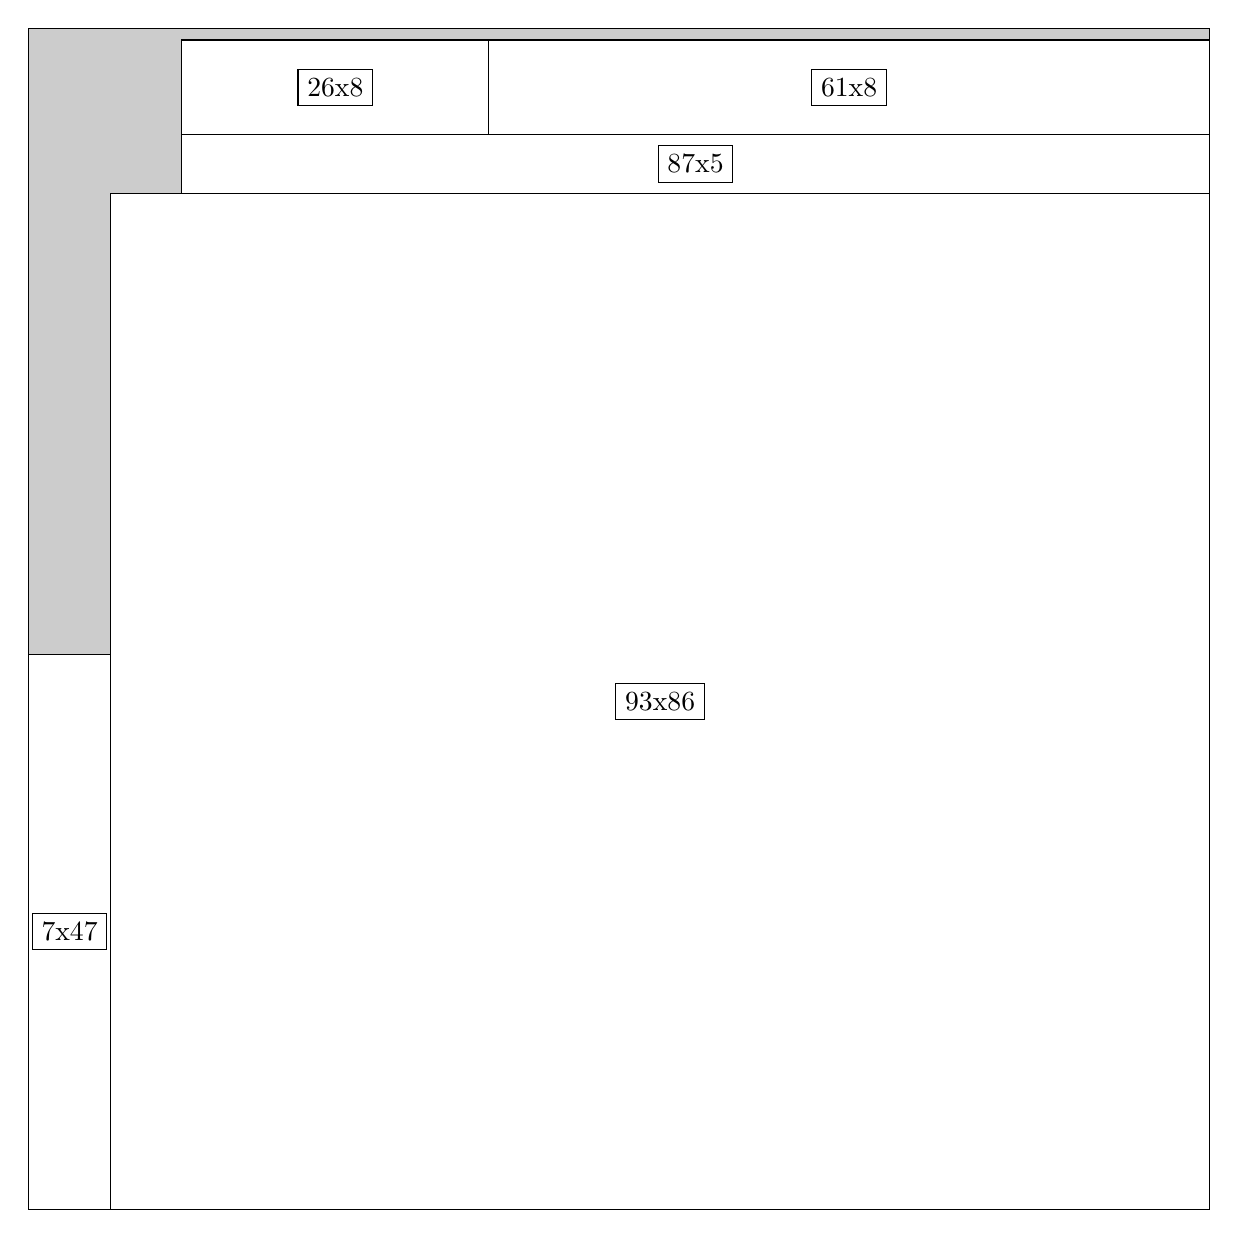
\begin{tikzpicture}[shorten >=1pt,scale=1.0,every node/.style={scale=1.0},->]
\tikzstyle{vertex}=[circle,fill=black!25,minimum size=14pt,inner sep=0pt]
\filldraw[fill=gray!40!white, draw=black] (0,0) rectangle (15.0,15.0);
\foreach \name/\x/\y/\w/\h in {93x86/1.05/0.0/13.95/12.9,87x5/1.95/12.9/13.049999999999999/0.75,61x8/5.85/13.65/9.15/1.2,26x8/1.95/13.65/3.9/1.2,7x47/0.0/0.0/1.05/7.05}
\filldraw[fill=white!40!white, draw=black] (\x,\y) rectangle node[draw] (\name) {\name} ++(\w,\h);
\end{tikzpicture}


w =93 , h =86 , x =7 , y =0 , v =7998
\par
w =87 , h =5 , x =13 , y =86 , v =435
\par
w =61 , h =8 , x =39 , y =91 , v =488
\par
w =26 , h =8 , x =13 , y =91 , v =208
\par
w =7 , h =47 , x =0 , y =0 , v =329
\par
\newpage


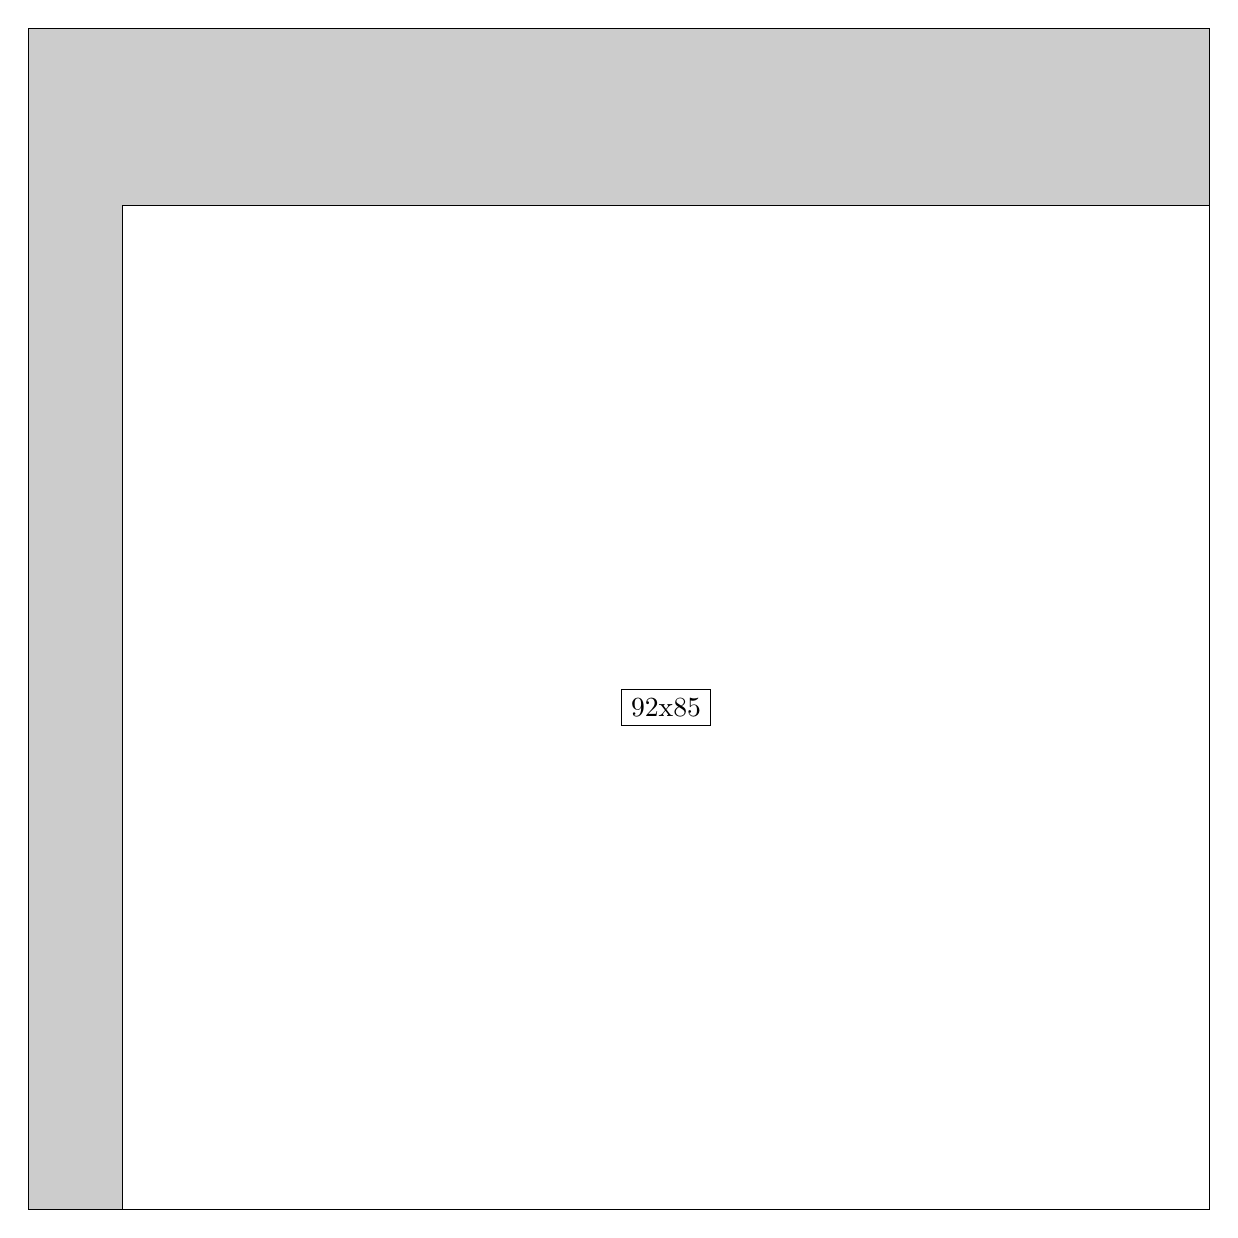
\begin{tikzpicture}[shorten >=1pt,scale=1.0,every node/.style={scale=1.0},->]
\tikzstyle{vertex}=[circle,fill=black!25,minimum size=14pt,inner sep=0pt]
\filldraw[fill=gray!40!white, draw=black] (0,0) rectangle (15.0,15.0);
\foreach \name/\x/\y/\w/\h in {92x85/1.2/0.0/13.799999999999999/12.75}
\filldraw[fill=white!40!white, draw=black] (\x,\y) rectangle node[draw] (\name) {\name} ++(\w,\h);
\end{tikzpicture}


w =92 , h =85 , x =8 , y =0 , v =7820
\par
\newpage


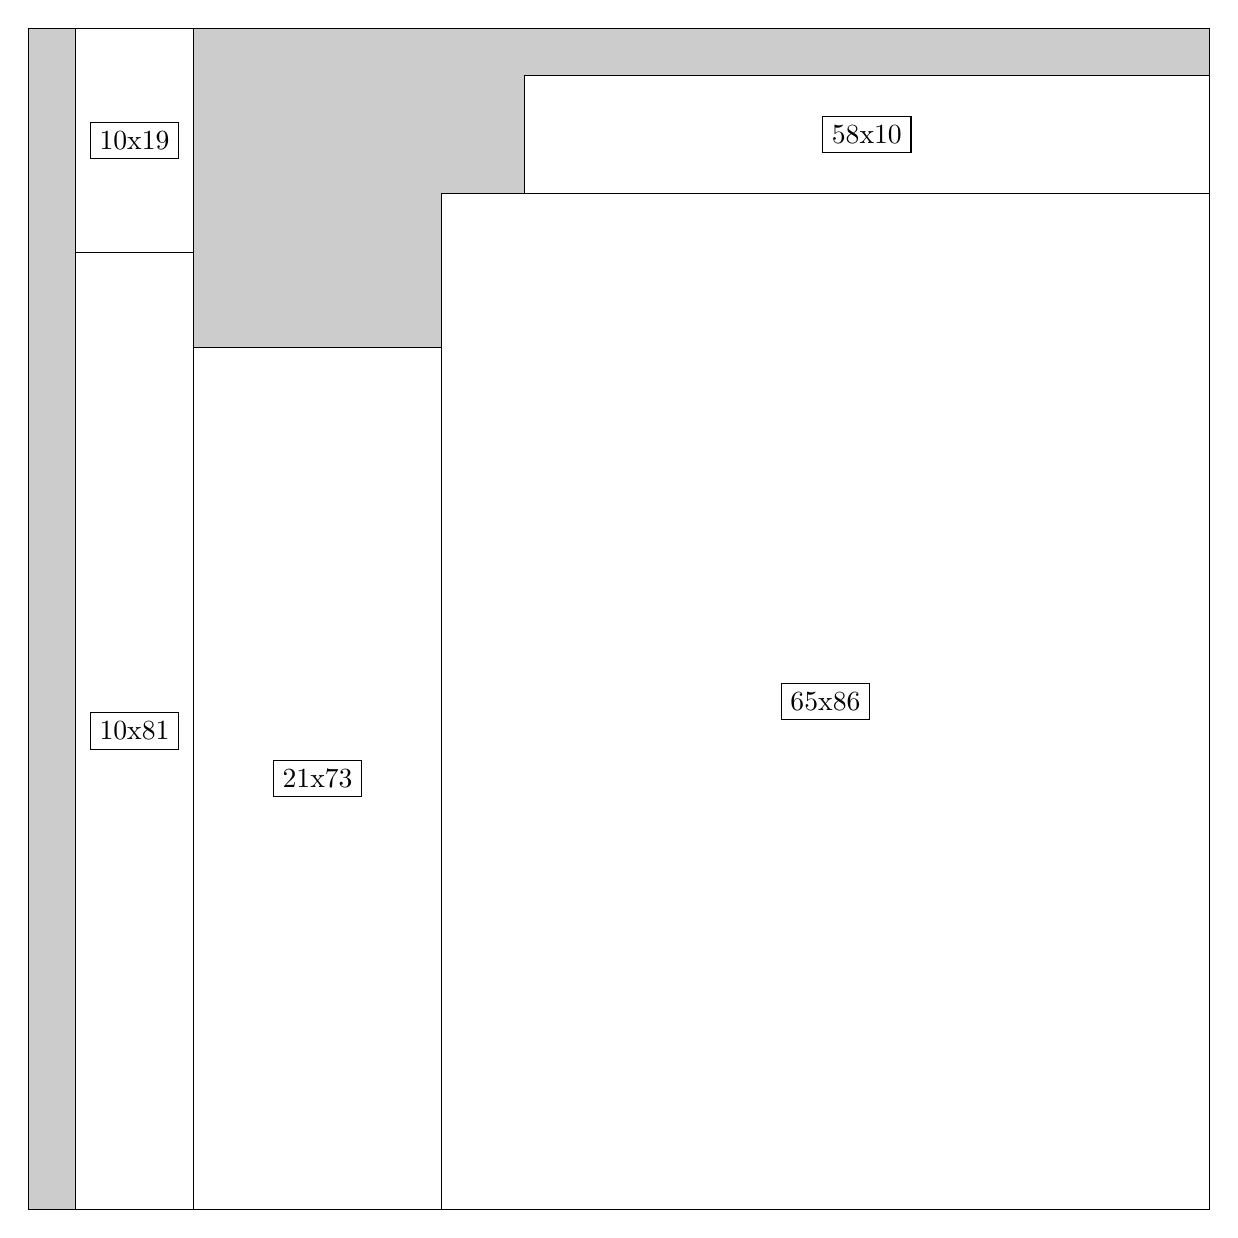
\begin{tikzpicture}[shorten >=1pt,scale=1.0,every node/.style={scale=1.0},->]
\tikzstyle{vertex}=[circle,fill=black!25,minimum size=14pt,inner sep=0pt]
\filldraw[fill=gray!40!white, draw=black] (0,0) rectangle (15.0,15.0);
\foreach \name/\x/\y/\w/\h in {65x86/5.25/0.0/9.75/12.9,58x10/6.3/12.9/8.7/1.5,21x73/2.1/0.0/3.15/10.95,10x81/0.6/0.0/1.5/12.15,10x19/0.6/12.15/1.5/2.85}
\filldraw[fill=white!40!white, draw=black] (\x,\y) rectangle node[draw] (\name) {\name} ++(\w,\h);
\end{tikzpicture}


w =65 , h =86 , x =35 , y =0 , v =5590
\par
w =58 , h =10 , x =42 , y =86 , v =580
\par
w =21 , h =73 , x =14 , y =0 , v =1533
\par
w =10 , h =81 , x =4 , y =0 , v =810
\par
w =10 , h =19 , x =4 , y =81 , v =190
\par
\newpage


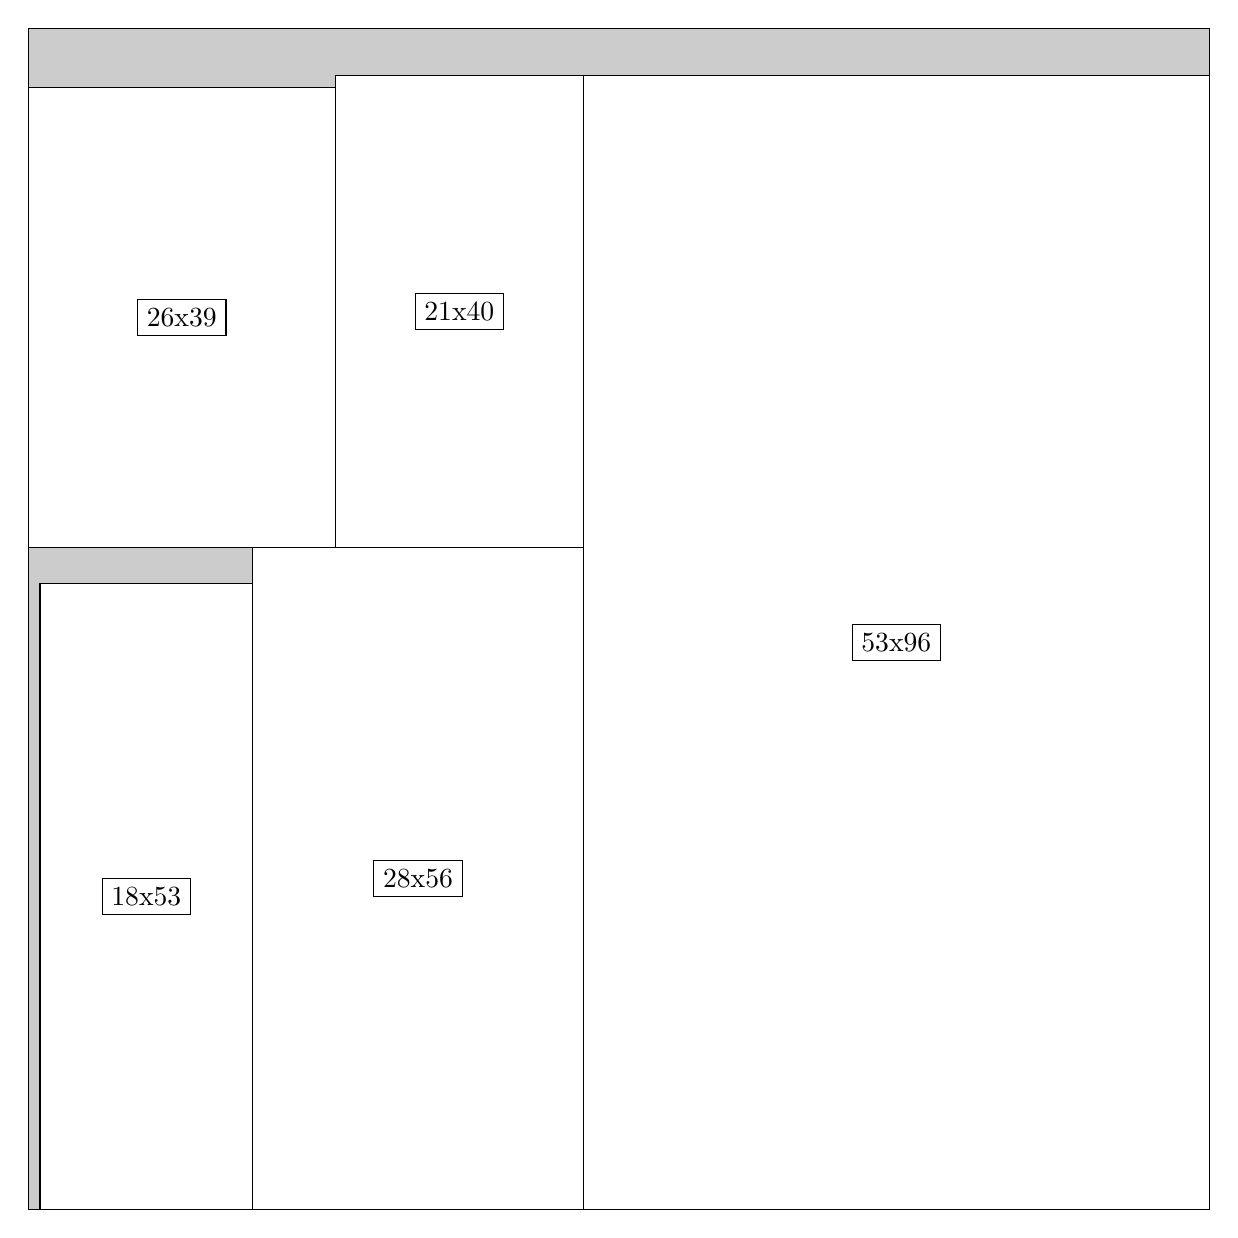
\begin{tikzpicture}[shorten >=1pt,scale=1.0,every node/.style={scale=1.0},->]
\tikzstyle{vertex}=[circle,fill=black!25,minimum size=14pt,inner sep=0pt]
\filldraw[fill=gray!40!white, draw=black] (0,0) rectangle (15.0,15.0);
\foreach \name/\x/\y/\w/\h in {53x96/7.05/0.0/7.949999999999999/14.399999999999999,28x56/2.85/0.0/4.2/8.4,18x53/0.15/0.0/2.6999999999999997/7.949999999999999,21x40/3.9/8.4/3.15/6.0,26x39/0.0/8.4/3.9/5.85}
\filldraw[fill=white!40!white, draw=black] (\x,\y) rectangle node[draw] (\name) {\name} ++(\w,\h);
\end{tikzpicture}


w =53 , h =96 , x =47 , y =0 , v =5088
\par
w =28 , h =56 , x =19 , y =0 , v =1568
\par
w =18 , h =53 , x =1 , y =0 , v =954
\par
w =21 , h =40 , x =26 , y =56 , v =840
\par
w =26 , h =39 , x =0 , y =56 , v =1014
\par
\newpage


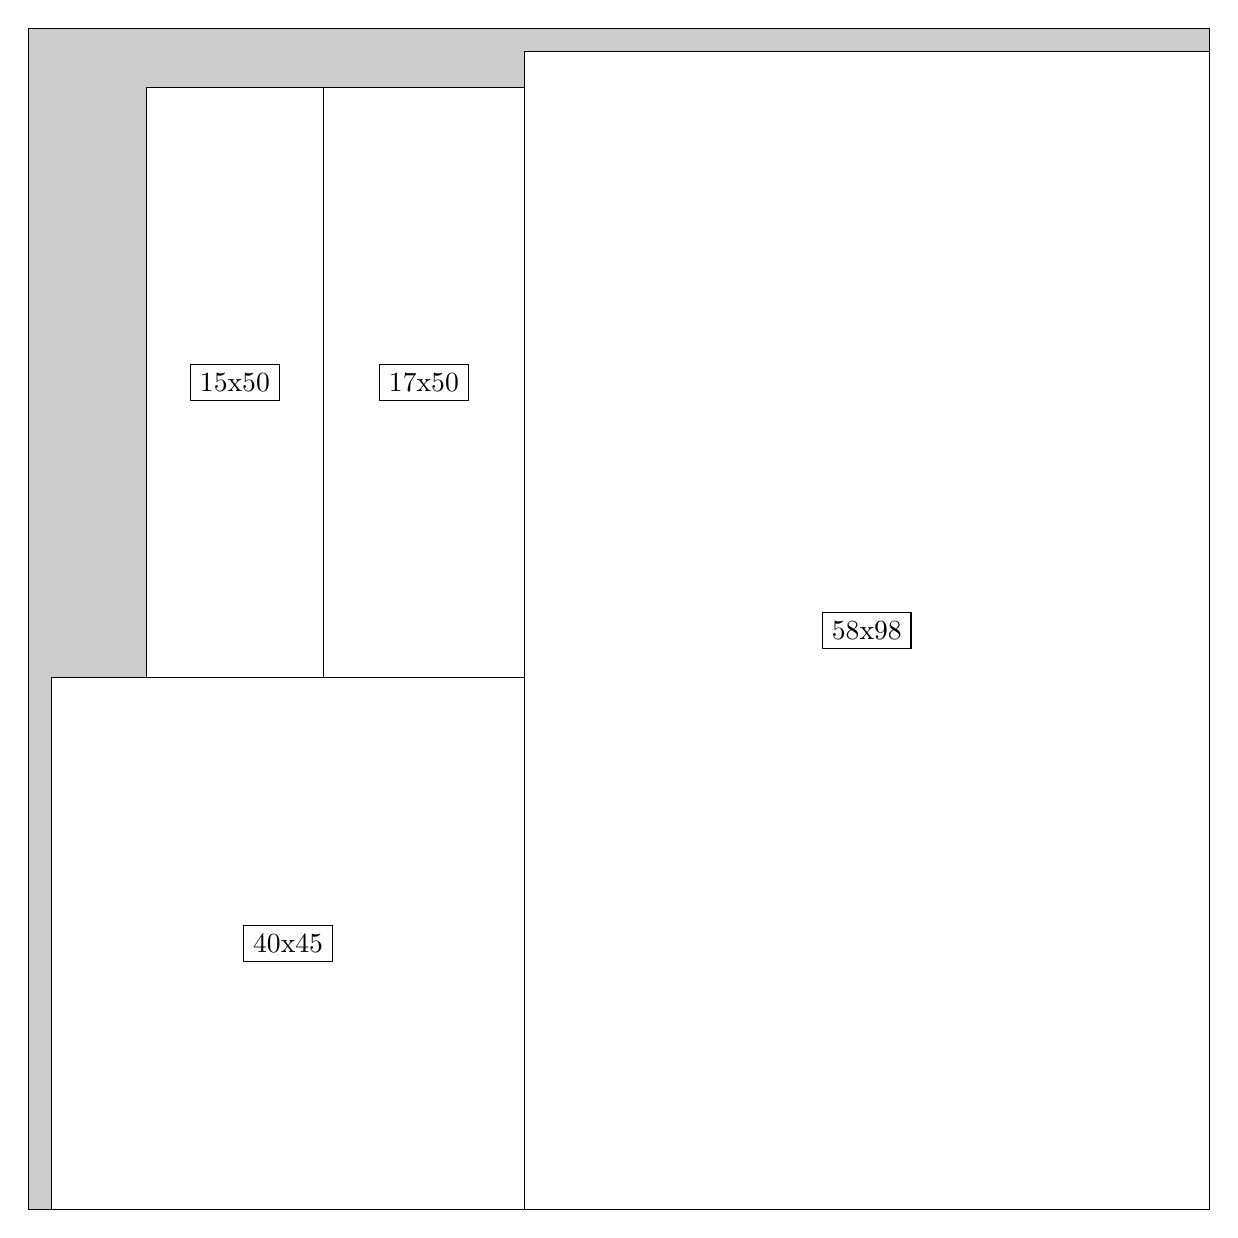
\begin{tikzpicture}[shorten >=1pt,scale=1.0,every node/.style={scale=1.0},->]
\tikzstyle{vertex}=[circle,fill=black!25,minimum size=14pt,inner sep=0pt]
\filldraw[fill=gray!40!white, draw=black] (0,0) rectangle (15.0,15.0);
\foreach \name/\x/\y/\w/\h in {58x98/6.3/0.0/8.7/14.7,40x45/0.3/0.0/6.0/6.75,17x50/3.75/6.75/2.55/7.5,15x50/1.5/6.75/2.25/7.5}
\filldraw[fill=white!40!white, draw=black] (\x,\y) rectangle node[draw] (\name) {\name} ++(\w,\h);
\end{tikzpicture}


w =58 , h =98 , x =42 , y =0 , v =5684
\par
w =40 , h =45 , x =2 , y =0 , v =1800
\par
w =17 , h =50 , x =25 , y =45 , v =850
\par
w =15 , h =50 , x =10 , y =45 , v =750
\par
\newpage


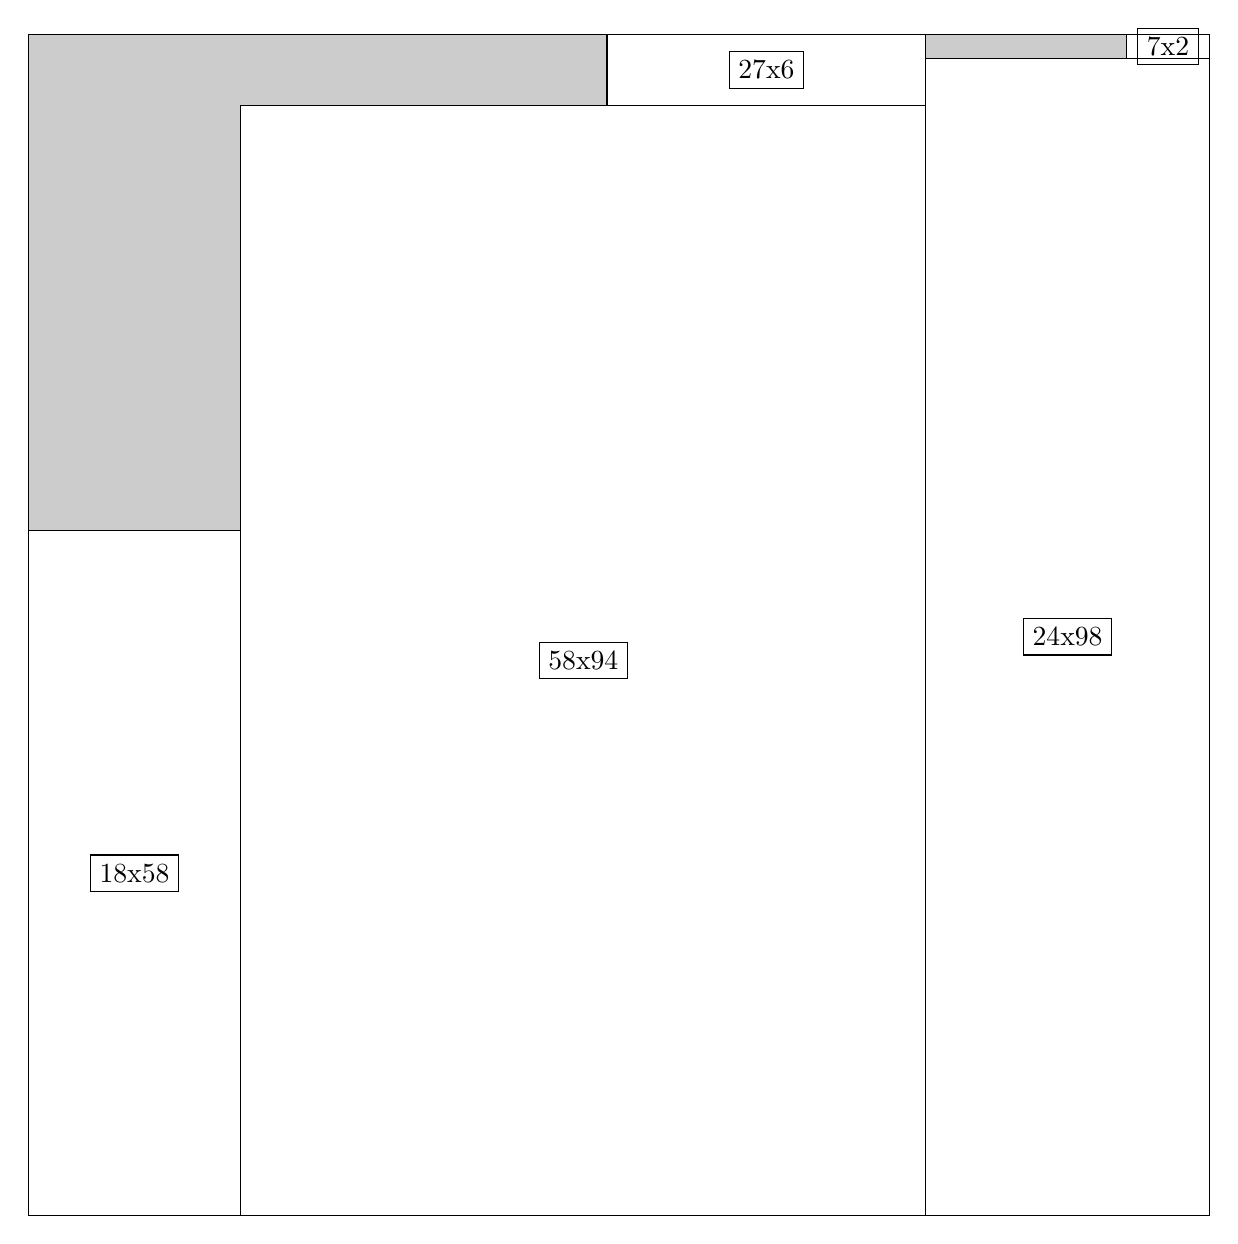
\begin{tikzpicture}[shorten >=1pt,scale=1.0,every node/.style={scale=1.0},->]
\tikzstyle{vertex}=[circle,fill=black!25,minimum size=14pt,inner sep=0pt]
\filldraw[fill=gray!40!white, draw=black] (0,0) rectangle (15.0,15.0);
\foreach \name/\x/\y/\w/\h in {24x98/11.4/0.0/3.5999999999999996/14.7,7x2/13.95/14.7/1.05/0.3,58x94/2.6999999999999997/0.0/8.7/14.1,27x6/7.35/14.1/4.05/0.8999999999999999,18x58/0.0/0.0/2.6999999999999997/8.7}
\filldraw[fill=white!40!white, draw=black] (\x,\y) rectangle node[draw] (\name) {\name} ++(\w,\h);
\end{tikzpicture}


w =24 , h =98 , x =76 , y =0 , v =2352
\par
w =7 , h =2 , x =93 , y =98 , v =14
\par
w =58 , h =94 , x =18 , y =0 , v =5452
\par
w =27 , h =6 , x =49 , y =94 , v =162
\par
w =18 , h =58 , x =0 , y =0 , v =1044
\par
\newpage


\end{document}